\subsection{Thiết kế cơ sở dữ liệu}

Trong kiến trúc microservice, mỗi dịch vụ quản lý một cơ sở dữ liệu độc lập theo đúng ranh giới domain. Vì vậy, mô hình dữ liệu không sử dụng quá nhiều ràng buộc khóa ngoại như kiến trúc nguyên khối. Thay vào đó, các quan hệ giữa dữ liệu được thể hiện ở mức logic hoặc thông qua các cơ chế đồng bộ sự kiện giữa các dịch vụ.

Như đã trình bày ở trên, hệ thống được xây dựng theo kiến trúc microservice trong đó có năm service dịch vụ được hiện thực bằng ngôn ngữ java cụ thể là user service, order service, product service, admin service và cart service. Mô hình ERD ban đầu được xây dựng dựa trên kiến trúc nguyên khối (monolithic) tổng thể, sau đó được phân tách và nhóm các thực thể cùng quan hệ tương ứng vào các CSDL riêng biệt dựa trên ranh giới của từng Microservice.

Service AI Agent (Python) được triển khai với Vector Database (Milvus), thay vì sử dụng PostgreSQL. Sự lựa chọn này là chiến lược, bởi vì Service AI cần lưu trữ và truy vấn các vector embeddings đa chiều hiệu suất cao, do đó, không sử dụng các mô hình ERD quan hệ truyền thống.

Hình \ref{fig:erd_overview} chính là sơ đồ ERD mô tả các thực thể và quan hệ giữa chúng trong từng service của hệ thống. Giới hạn của mỗi service được mô tả bằng một vùng màu khác nhau để dễ phân biệt và rạch ròi hơn, cụ thể màu xanh dương là user service, cam cho order service, vàng cho product service, admin service được vẽ trong vùng màu tím, và vùng xanh lá là cart service. 

\begin{figure}[H]
    \centering
    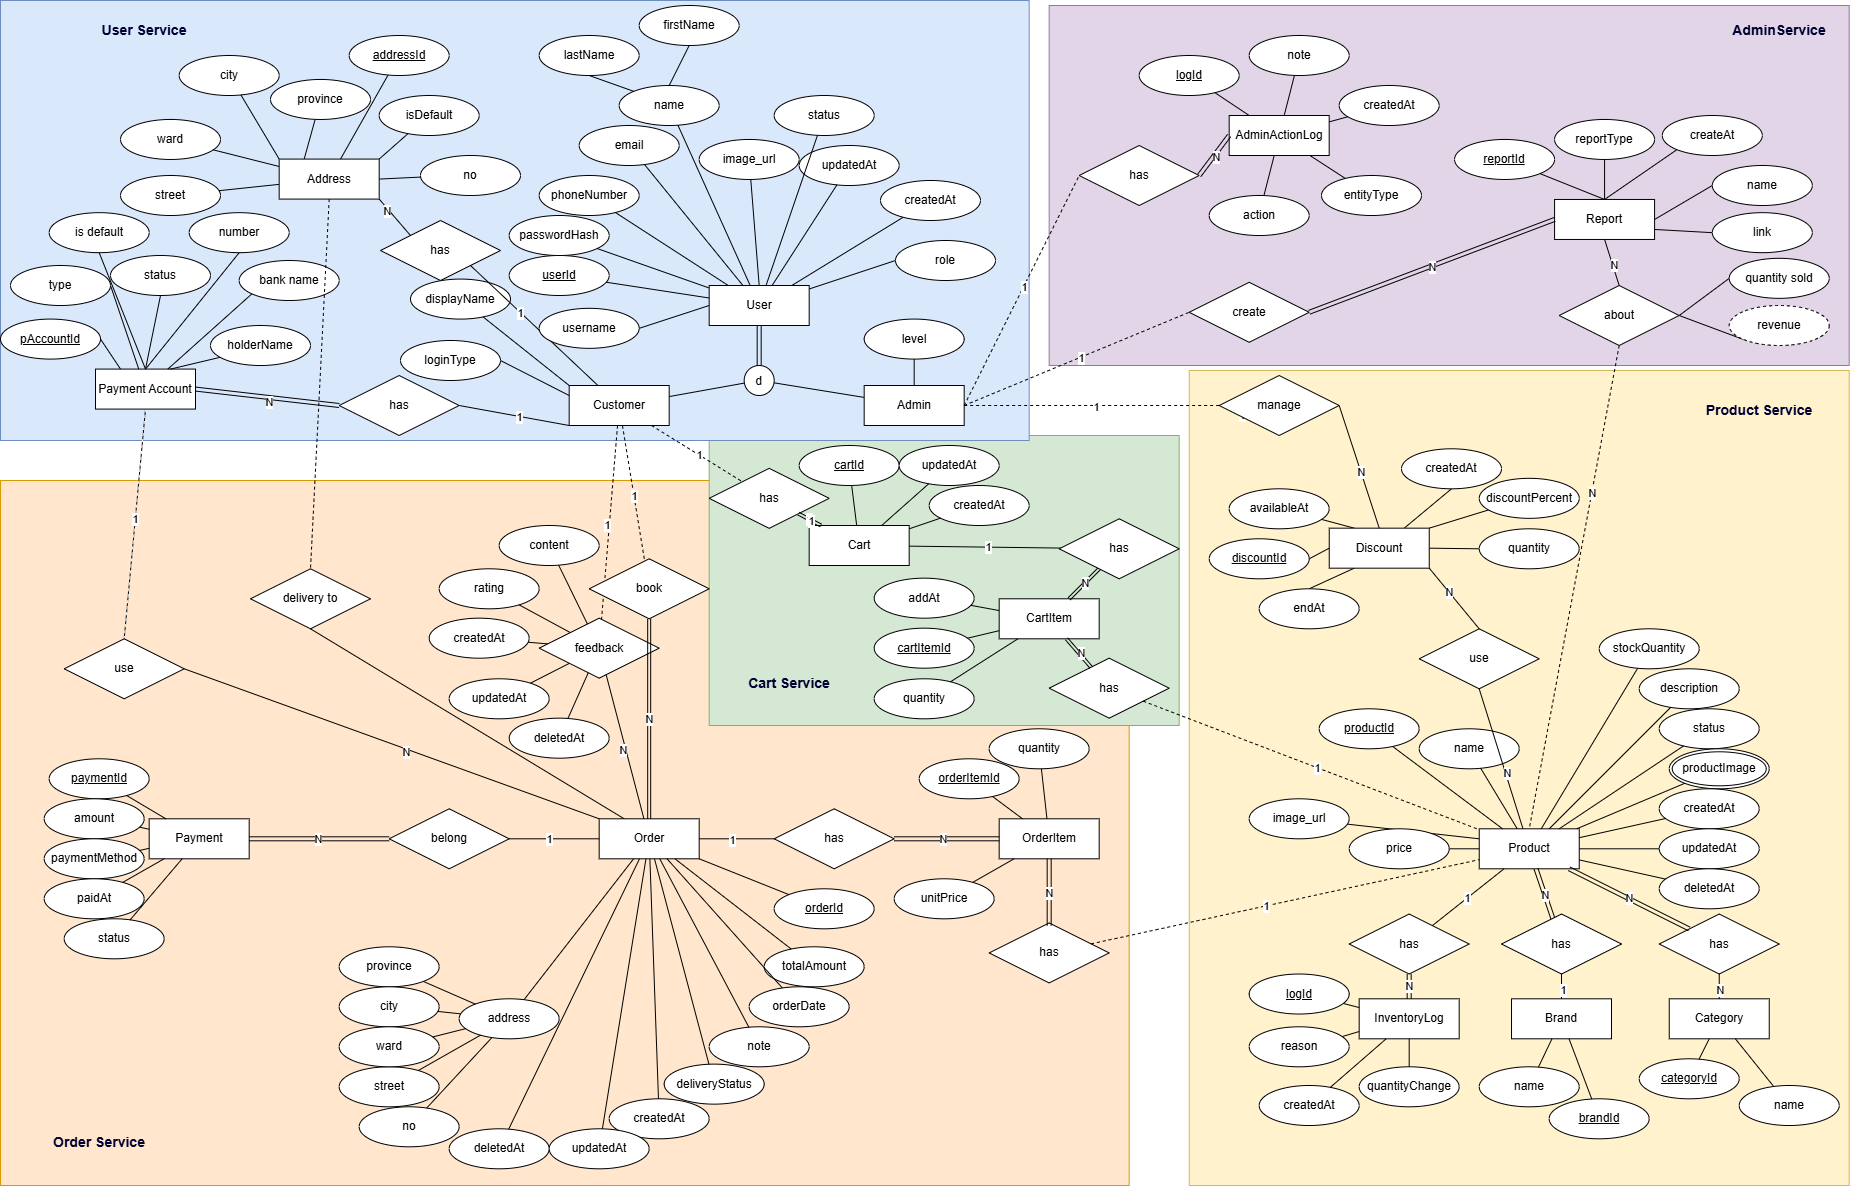
\includegraphics[width=0.9\linewidth]{images/chap6/erd/erd.png}
    \vspace{0.5cm}
    \caption{Sơ đồ ERD}
    \label{fig:erd_overview}
\end{figure}

Sơ đồ ERD tổng quan mô tả các thực thể chính của từng domain trong hệ thống. Mỗi nhóm thực thể được tổ chức tách biệt theo chức năng. Các mối quan hệ giữa chúng chỉ mang tính chất tham chiếu logic nhằm mô tả dòng dữ liệu, không phải là ràng buộc vật lý trong cơ sở dữ liệu.

\begin{figure}[H]
    \centering
    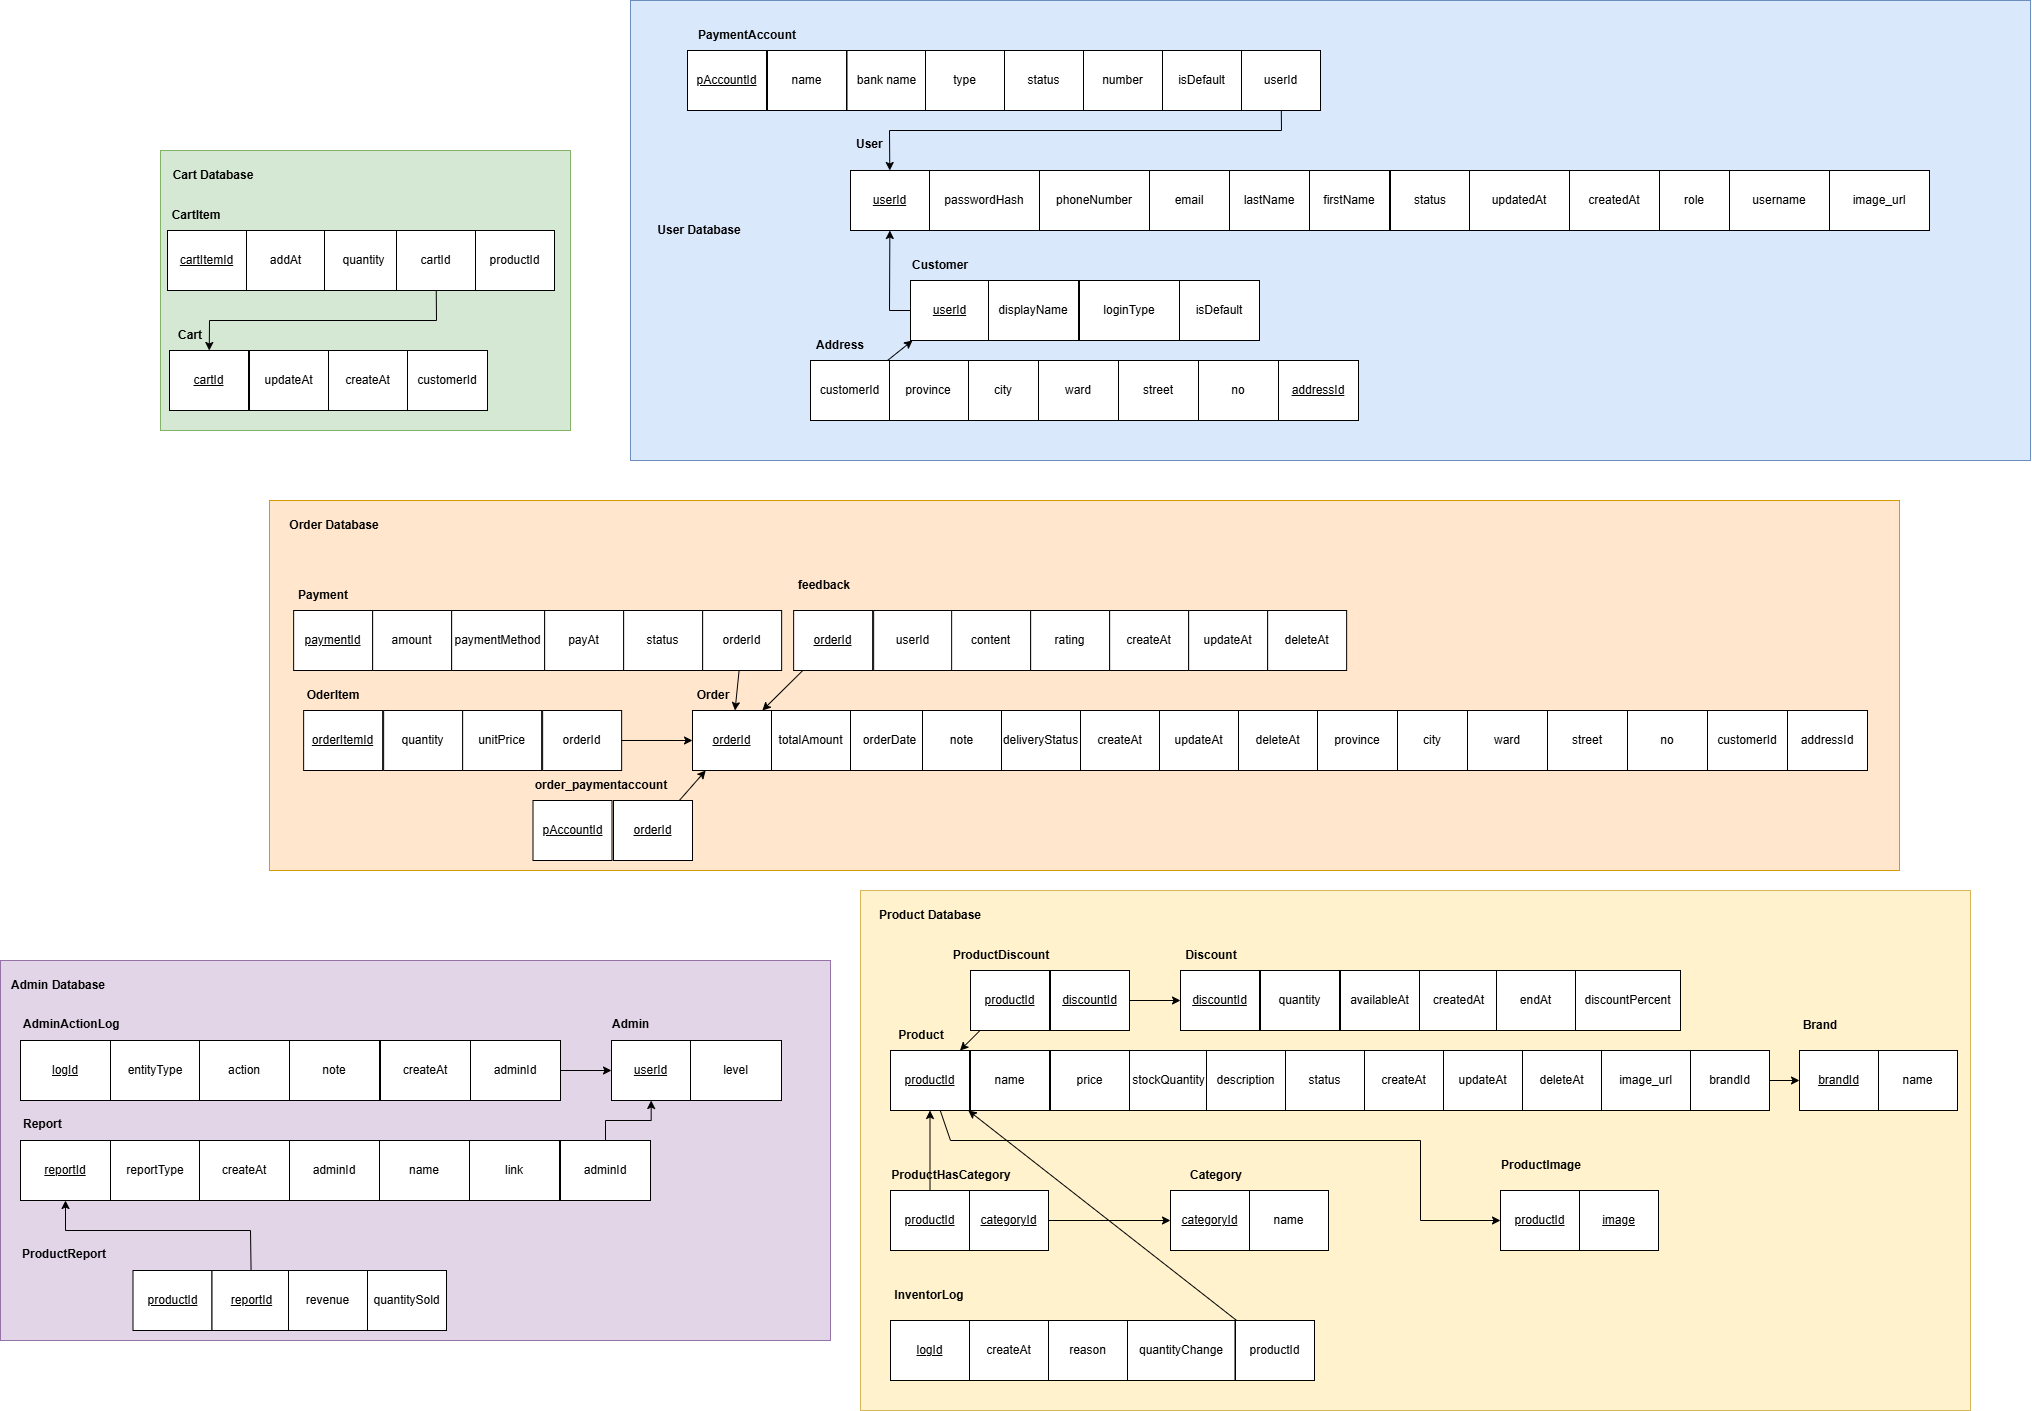
\includegraphics[width=0.9\linewidth]{images/chap6/erd/erd_mapping.png}
    \vspace{0.5cm}
    \caption{Sơ đồ ánh xạ ERD}
    \label{fig:erd_mapping}
\end{figure}

Hình \ref{fig:erd_mapping} biểu diễn sơ đồ ánh xạ ERD đã mô tả cách các thực thể được chuyển đổi sang mô hình lưu trữ trong từng microservice. Thay vì sử dụng khóa ngoại, mỗi bảng lưu trữ các định danh cần thiết để hỗ trợ giao tiếp giữa các dịch vụ hoặc đồng bộ dữ liệu. Cách tiếp cận này giúp hệ thống linh hoạt hơn, dễ mở rộng và phù hợp với các mô hình giao tiếp như event-driven và API orchestration.

Để cụ thể hơn cho từng service, các phần dưới đây sẽ trình bày chi tiết về các thực thể và quan hệ nội bộ trong từng ranh giới domain của năm dịch vụ cốt lõi sử dụng CSDL quan hệ PostgreSQL.

\subsubsection{ERD chi tiết cho user service}

Hình \ref{fig:user-service} bên dưới chính là ERD chi tiết cho user service, nó mô tả chi tiết các entity và quan hệ bên trong nội bộ service.

User Service là domain chịu trách nhiệm quản lý danh tính và thông tin giao dịch cá nhân của tất cả người dùng trong hệ thống. Thực thể User đóng vai trò là cốt lõi, lưu trữ các thông tin định danh và có quan hệ disjoint để phân loại rõ ràng giữa Customer  và Admin, thể hiện sự phân quyền trong hệ thống.

Thực thể Customer mở rộng vai trò của người dùng thông thường và là trung tâm của các quan hệ giao dịch cá nhân. Mỗi Khách hàng có quan hệ 1:N với thực thể Address, cho phép lưu trữ nhiều địa chỉ giao hàng khác nhau. Đồng thời, Khách hàng cũng có quan hệ 1:N với thực thể Payment Account, quản lý các phương thức thanh toán đã liên kết.

\begin{figure}[H]
    \centering
    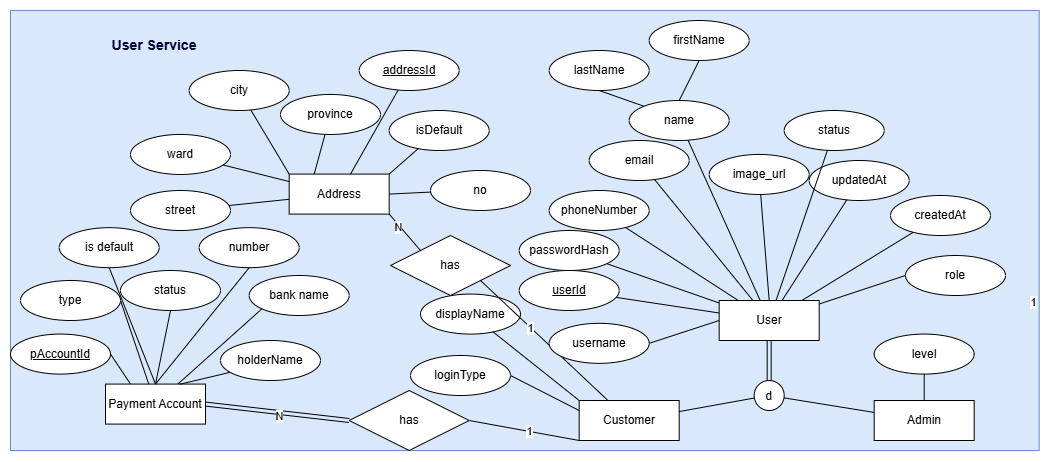
\includegraphics[width=1\linewidth]{images/chap6/erd/user-service.png}
    \vspace{0.5cm}
    \caption{ERD chi tiêt cho user service}
    \label{fig:user-service}
\end{figure}

User service độc lập và chỉ quản lý các thực thể thuộc phạm vi người dùng. Mọi service khác trong kiến trúc Microservice, như Order Service, sẽ chỉ tham chiếu đến dữ liệu này bằng ID (ví dụ: userId, addressId) mà không cần lưu trữ lại thông tin chi tiết.

\subsubsection{ERD chi tiết cho order service}

Order Service chịu trách nhiệm xử lý toàn bộ vòng đời của một giao dịch mua hàng, bao gồm việc quản lý đặt hàng, thanh toán, và phản hồi từ khách hàng. Thiết kế dữ liệu xoay quanh thực thể Order. Order lưu trữ thông tin tổng quan về giao dịch và địa chỉ giao hàng chi tiết (no, street, city, province) để đảm bảo tính bất biến của đơn hàng tại thời điểm đặt.

Thực thể Order có quan hệ 1:N với OrderItem, cho phép Order Service quản lý các mặt hàng được mua cùng số lượng và giá cả cụ thể. Đồng thời, mỗi Đơn hàng được liên kết 1:1 với thực thể Payment để theo dõi thông tin và trạng thái giao dịch tiền tệ liên quan. Ngoài ra, Order cũng có quan hệ với thực thể Feedback, cho phép khách hàng thực hiện đánh giá sau khi hoàn tất đơn hàng.

Hình \ref{fig:order-service} chính là ERD chi tiết của order service. Qua hình \ref{fig:order-service} cho thấy order Service được thiết kế để tách biệt vật lý khỏi các service khác. Các quan hệ ngoại lai được thể hiện trên sơ đồ nhằm mục đích minh họa các khóa ngoại logic:

\begin{itemize}
    \item Quan hệ \textbf{use} từ Order: tham chiếu đến thực thể Payent Account (user service), cho biết khách hàng đã dùng tài khoản nào để thanh toán cho đơn hàng.
    \item Quan hệ \textbf{deliver to} từ Order: tham chiếu đến thực thể Address (user service), cho biết đơn hàng được giao đến địa chỉ cụ thể nào của khách hàng.
    \item Quan hệ \textbf{book} từ Order: tham chiếu đến thực thể Customer(user service), thể hiện được khách hàng nào đã đặt đơn hàng.
    \item Quan hệ \textbf{feedback} từ Order: tham chiếu đến thực thể Customer(user service), lưu lại những đánh giá của khách hàng dành cho đơn hàng của họ.
    \item Quan hệ \textbf{has} từ OrderItem: tham chiếu đến thực thể Product(product service),chỉ ra sản phẩm nào đã được mua.
\end{itemize}

\begin{figure}[H]
    \centering
    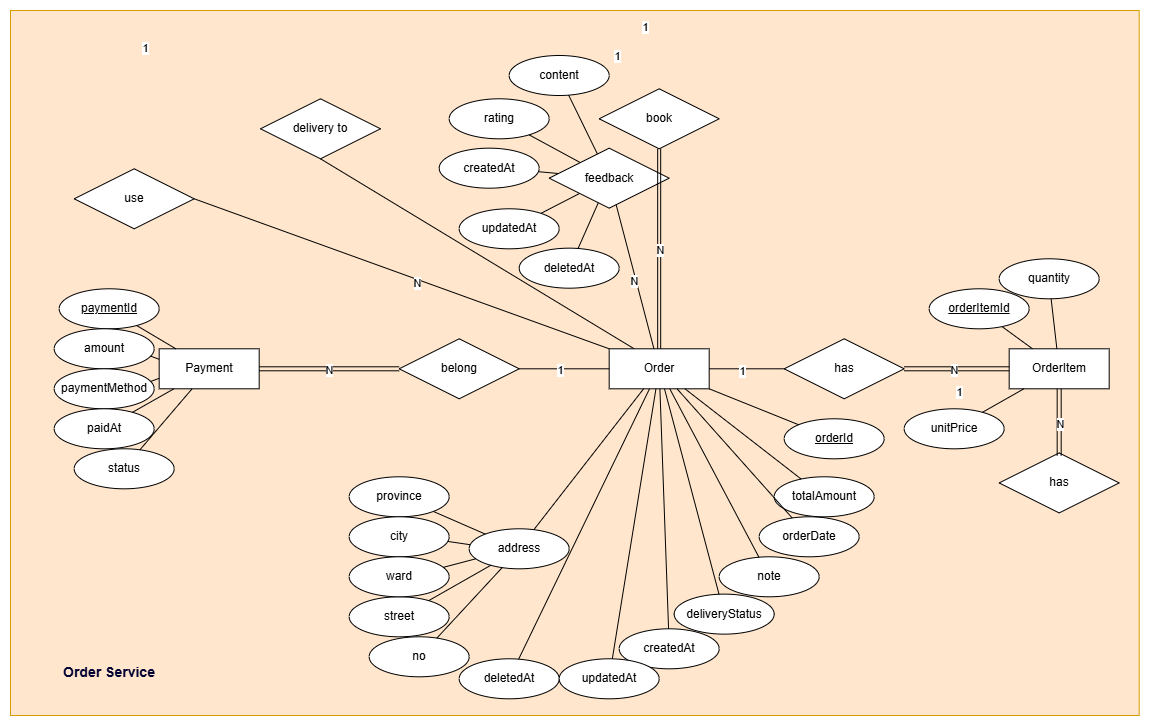
\includegraphics[width=1\linewidth]{images/chap6/erd/order-service.png}
    \vspace{0.5cm}
    \caption{ERD chi tiêt của order service}
    \label{fig:order-service}
\end{figure}

Trong thực tế, Order Service sẽ chỉ lưu trữ các ID ngoại lai (như UserID hoặc ProductID) mà không có ràng buộc khóa ngoại vật lý, nhằm duy trì tính độc lập (autonomy) và khả năng phục hồi của CSDL theo đúng kiến trúc Microservice.

\subsubsection{ERD chi tiết cho product service}

Product Service là domain cốt lõi chịu trách nhiệm quản lý toàn bộ dữ liệu danh mục sản phẩm, bao gồm các thông tin liên quan đến tồn kho, thương hiệu, phân loại, và khuyến mãi. Thiết kế dữ liệu xoay quanh thực thể Product.

Thực thể Product là trung tâm, lưu trữ các thông tin chi tiết như tên, giá cả, mô tả và số lượng tồn kho (stockQuantity). Product có quan hệ N:1 với thực thể Brand và Category,  giúp phân loại và tổ chức sản phẩm một cách logic. Để kiểm soát hàng hóa, Product có quan hệ 1:N với InventoryLog, nơi ghi lại mọi sự thay đổi về số lượng tồn kho và lý do.

Ngoài ra, dịch vụ này còn quản lý các chương trình Discount. Khuyến mãi có quan hệ N:M (nhiều-nhiều) với Product, cho phép cùng một lúc nhiều sản phẩm có thể áp dụng nhiều chương trình giảm giá khác nhau.

Hình \ref{fig:order-service} chính là ERD chi tiết của order service. Qua sơ đồ ở hình \ref{fig:product-service} quan hệ \textbf{manage} từ Discount tham chiếu đến thực thể Admin (user service) thể hiện quản trị viên đã tạo hay chỉnh sửa giảm giá.

\begin{figure}[H]
    \centering
    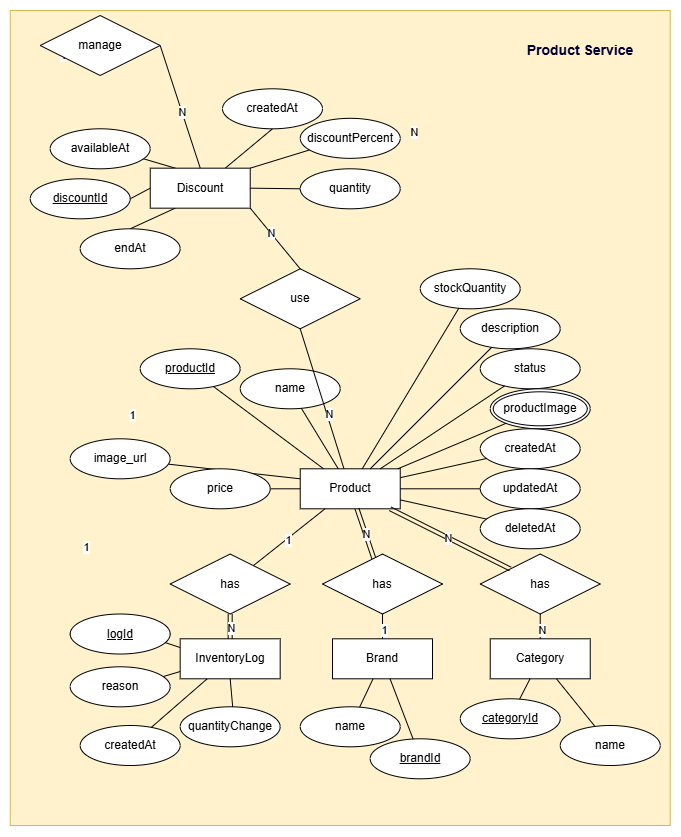
\includegraphics[width=0.6\linewidth]{images/chap6/erd/product-service.png}
    \vspace{0.5cm}
    \caption{ERD chi tiêt của product service}
    \label{fig:product-service}
\end{figure}

Product service là một trong những nguồn dữ liệu quan trọng nhất của hệ thống và được các service khác tham chiếu đến. Order service và cart service sử dụng khóa ngoại logic (ProductID) để xác định sản phẩm. Khi có sự thay đổi về giá cả hoặc tồn kho, product service chịu trách nhiệm phát hành các sự kiện lên Apache Kafka để đồng bộ hóa dữ liệu với các service tiêu thụ khác.

\subsubsection{ERD chi tiết cho cart service}

Cart Service là domain có thiết kế tối giản, tập trung vào việc quản lý trạng thái giỏ hàng tạm thời của khách hàng. Dịch vụ này cần duy trì hiệu suất cao vì nó xử lý các thao tác đọc/ghi thường xuyên. Thiết kế dữ liệu xoay quanh thực thể Cart, đại diện cho một giỏ hàng của khách hàng.

Thực thể Cart có quan hệ 1:N với CartItem. CartItem lưu trữ thông tin về các mặt hàng cụ thể mà khách hàng đã thêm vào giỏ, bao gồm số lượng (quantity) và thời gian thêm (addAt).

Hình \ref{fig:cart-service} bên dưới mô tả các entity và các quan hệ ngoại lại của cart service. Cart service có hai tham chiếu ngoại lai chính:

\begin{itemize}
    \item Quan hệ \textbf{has} từ Cart: tham chiếu đến thực thể Customer (user service) để xác định chủ nhân của giỏ hàng.
    \item Quan hệ \textbf{has} từ CartItem: tham chiếu đến thực thể Product (product service) để biết thông tin về mặt hàng được chọn.
\end{itemize}

\begin{figure}[H]
    \centering
    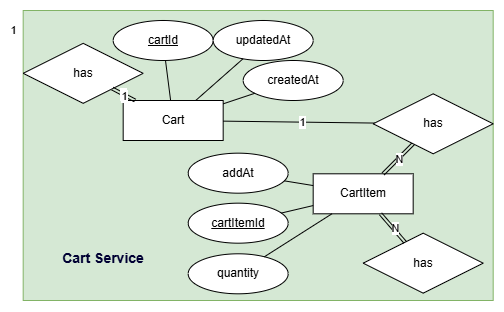
\includegraphics[width=0.6\linewidth]{images/chap6/erd/cart-service.png}
    \vspace{0.5cm}
    \caption{ERD chi tiêt của cart service}
    \label{fig:cart-service}
\end{figure}

\subsubsection{ERD chi tiết cho admin service}

Admin Service là domain phụ trợ, có vai trò cốt lõi là duy trì tính minh bạch (accountability) của các hành động quản trị và quản lý các báo cáo thống kê của hệ thống. Dịch vụ này được thiết kế với hai thực thể chính.

Thực thể AdminActionLog là thành phần quan trọng để theo dõi và ghi lại mọi thao tác quan trọng do Admin thực hiện, bao gồm action (hành động đã làm), entityType (thực thể bị ảnh hưởng). Thêm vào đó, thực thể Report chịu trách nhiệm lưu trữ và quản lý các báo cáo thống kê và phân tích hiệu suất, bao gồm loại báo cáo (reportType), tên và các chỉ số hiệu suất (revenue, quantity sold).

Các entity và quan hệ của admin service được miêu tả cụ thể trong hình \ref{fig:admin-service}. Qua hình \ref{fig:admin-service}, ta thấy được admin service có ba quan hệ ngoại lại chính:

\begin{itemize}
    \item Quan hệ \textbf{has} từ AdminActionLog: tham chiếu đến Admin (user service), xác định quản trị viên đã thực hiện hành động.
    \item Quan hệ \textbf{create} từ Report: tham chiếu đến Admin (user service), xác định quản trị viên đã tạo báo cáo.
    \item Quan hệ \textbf{about} từ Report: tham chiếu đến Product (product service), cho biết báo cáo đó thống kê về các sản phẩm nào.
\end{itemize}

\begin{figure}[H]
    \centering
    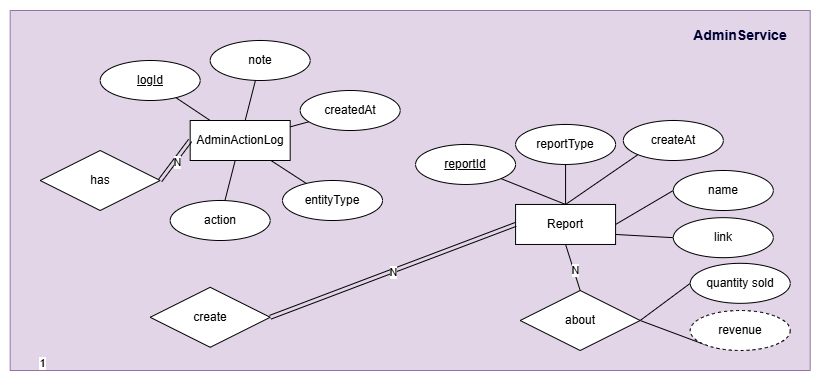
\includegraphics[width=0.9\linewidth]{images/chap6/erd/admin-service.png}
    \vspace{0.5cm}
    \caption{ERD chi tiêt của admin service}
    \label{fig:admin-service}
\end{figure}
